%!TEX root = ../main.tex

\section{\texorpdfstring{$\CP$}{CP} violation in \texorpdfstring{$\bToccbard$}{bToccbard} decays}
\label{sec:cpviolation:btoccbard}

The decay \BdToDD can be described with the Feynman diagrams in
\cref{fig:cpviolation:feynmandiagrams_bdtodd}.
\begin{figure}[htb]
\centering
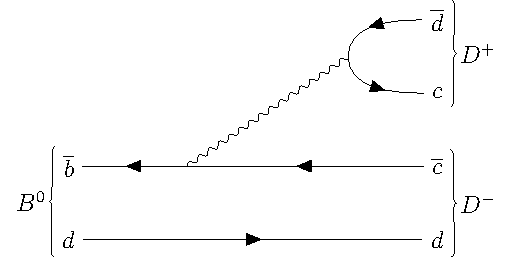
\includegraphics[width=0.48\textwidth]{03-CPViolation/tikz/pdf/BdToDD_Tree.pdf}
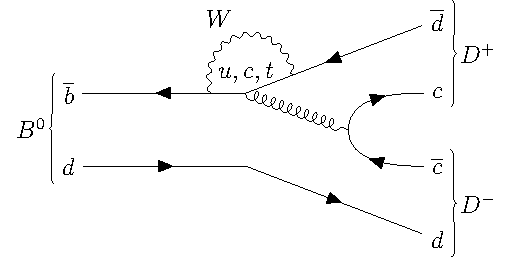
\includegraphics[width=0.48\textwidth]{03-CPViolation/tikz/pdf/BdToDD_Penguin.pdf}
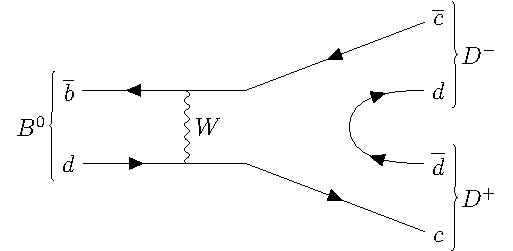
\includegraphics[width=0.48\textwidth]{03-CPViolation/tikz/pdf/BdToDD_Exchange.pdf}
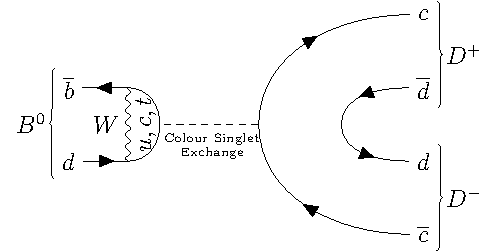
\includegraphics[width=0.48\textwidth]{03-CPViolation/tikz/pdf/BdToDD_Annihilation.pdf}
\caption{Main Feynman diagrams contributing to \BdToDD decays. Apart from the
tree diagram (top left), a penguin diagram (top right), an exchange diagram
(bottom left) and a penguin annihilation diagram (bottom right) are shown.}
\label{fig:cpviolation:feynmandiagrams_bdtodd}
\end{figure}
The tree diagram ($T$) proceeds via a \bToccbard quark transition, which is
CKM suppressed. The contributions from the other diagrams, especially the
penguin diagrams ($P^{(q)}$ with $q = \cquark$ and \tquark quarks in the
loop), but also exchange ($E$) and penguin annihilation diagrams
($P\!A^{(q)}$), need to be taken into account as well because they can carry
different weak phases and are not Cabibbo-suppressed. Thus, the decay
amplitude is given by~\cite{Fleischer1999,Fleischer2007,Bel:2015wha}
\begin{align}
	A(\BdToDD) = \Vcb \mathcal{A}[1 - ae^{i\theta}e^{i\gamma}]\,,
\end{align}
with
\begin{align}
	\mathcal{A} \equiv \Vcds[T + E + {P^{(c)} + P\!A^{(c)}} - {P^{(t)} + P\!A^{(t)}}]\,,
\end{align}
and
\begin{align}
	ae^{i\theta} \equiv R_b\left[\frac{{P^{(u)} + P\!A^{(u)}} - {P^{(t)} + P\!A^{(t)}}}{T + E + {{P^{(c)} + P\!A^{(c)}} - {P^{(t)} + P\!A^{(t)}}}}\right]\,.
\end{align}
Here, $R_b$ is a side length of the unitarity triangle defined in
\cref{eq:cpviolation:Rb}. The angle $\gamma$ of the unitarity triangle is a
\CP-violating weak phase, while $a$ and $\theta$ are hadronic \CP-conserving
parameters. Therefore, the corresponding \Bzb decay amplitude is
\begin{align}
	A(\BdbToDD) = \Vcbs \mathcal{A}[1 - ae^{i\theta}e^{-i\gamma}]\,.
\end{align}
The parameter describing \CP violation in the interference can be written as
\begin{align}
\begin{split}
	\lambda_{\Dp\Dm} &= \frac{\Vtbs\Vtd}{\Vtb\Vtds}\frac{\Vcb\Vcds}{\Vcbs\Vcd}\frac{1-ae^{i\theta}e^{i\gamma}}{1-ae^{i\theta}e^{-i\gamma}}\,,\\
					 &= e^{-i2\beta}\frac{1-ae^{i\theta}e^{i\gamma}}{1-ae^{i\theta}e^{-i\gamma}}\,,
\end{split}
\end{align}
using the ratio of the mixing coefficients from
\cref{eq:cpviolation:qp_simplified} and the definition of the unitarity
triangle $\beta$ from \cref{eq:cpviolation:angles}. Different than for
\BdToJPsiKS (cf.~\cref{eq:lambda_JPsiKS}) the \CP eigenvalue is $\eta_{\CP} =
\num{+1}$, since no spins are involved in the decay \BdToDD. The hadronic
parameters cannot be calculated reliably within QCD~\cite{Bel:2015wha}. Thus,
they must be determined through a measurement of the \CP observables, which
can be expressed via
\begin{align}
	\SDD &= -\frac{\sin\phid - 2a \cos\theta\sin(\phid + \gamma) + a^2\sin(\phid + 2\gamma)}{1 - 2a\cos\theta\cos\gamma + a^2}\,,\\
	\CDD &= \frac{2a\sin\theta\sin\gamma}{1 - 2a\cos\theta\cos\gamma + a^2}\,.
\end{align}
The term \SDD gives access to the mixing phase \phid, which is related to $\beta$ through
\begin{align}
	\phid = 2\beta + \phi_d^{\mathrm{NP}}\,,
\end{align}
and thus considers new physics contributions as well. While \SDD is caused by
interference between the direct decay and the decay after mixing, \CDD
might differ from zero due to interferences between tree and penguin
contributions. Different than in the case of \BdToJPsiKS only an effective
phase
\begin{align}
	\phideff = \phid + \Delta\phid
\end{align}
with
\begin{align}
	\sin\phideff = -\frac{\SDD}{\sqrt{1 - \CDD^2}}
\end{align}
can be measured in \BdToDD. The phase shift $\Delta\phi$ is given by
\begin{align}
	\tan\Delta\phi = \frac{a^2\sin2\gamma - 2a\cos\theta\sin\gamma}{1 - 2a\cos\rho\cos\gamma + a^2\cos2\gamma}\,.
\end{align}

The decay channel \BsToDsDs is also governed by a \bToccbard transition. It
gives access to \phis. However, the measurement is as well polluted by
hadronic penguin effects. Since \BsToDsDs is related to \BdToDD via U-spin
symmetry, the phase shift $\Delta\phi$ can be transferred.

Further decay modes from the family of \BToDDbar decays are \BdToDstD and
\BdToDstDst, which also enable a determination of \phideff, but introduce
further complications. For \BdToDstD the final state is no \CP eigenstate as
it can be distinguished by the charge of the \Dstarpm meson. Thus, four \CP
observables are needed to describe \CP violation. Furthermore, from an
experimentalist's point of view the final state is not symmetrical in terms of
the charges of pions and kaons and thus a detection asymmetry has to be taken
into account. In the measurement of \CP violation using \BdToDstDst decays,
like for \BsToJPsiPhi decays, an angular-dependent analysis is required.
